\documentclass[12pt,letterpaper,english]{article}
\usepackage[T1]{fontenc}
\usepackage[latin9]{inputenc}
\pagestyle{empty}
\usepackage{amsmath}
\usepackage{amssymb}
\usepackage{graphicx}
\usepackage{bm}
\usepackage{multicol}
\usepackage{enumitem}

\usepackage{hyperref}
\hypersetup{
    colorlinks=true,
    linkcolor=blue,
    filecolor=magenta,      
    urlcolor=cyan,
}


\newcommand{\norm}[1]{\lVert#1\rVert}

\makeatletter

\special{papersize=\the\paperwidth,\the\paperheight}



\textwidth6.5in\textheight9in\topmargin-.25in\oddsidemargin0in\evensidemargin0in\parskip5pt\parindent0pt



\usepackage{fancyhdr}
\pagestyle{fancy}
\lhead{Reconfigurable Mechanical Vibrations Laboratory Kit}
\rhead{}


\usepackage{lastpage}
 
  
\rfoot{Page \thepage \hspace{1pt} of \pageref{LastPage}}

%\rfoot{\small }
\lfoot{Mechanical Vibrations: Lab 4}
\cfoot{}




\usepackage{babel}


\makeatother

\usepackage{babel}
\begin{document}
\global\long\def\Re{{\rm {Re }}}
 \global\long\def\cL{{\cal L}}
 \global\long\def\sq{{\rm {sq}}}
 \global\long\def\bfx{{\bf x}}
 \global\long\def\bfi{{\bf i}}
 \global\long\def\bfj{{\bf j}}
 
 


\begin{center}
\textbf{\large Lab Assignment 4: Multi-DOF Systems}
\par\end{center}{\large \par}

The goal of this demo will be to explore a two degree of freedom system consisting of two springs and two masses. First, read through section E1 (``1 DOF and 2 DOF Assembly'') in the Assembly Guide in order to set up the system.  Note that this setup for this lab is identical to the first lab (1DOF) with the exception of an extra spring and nut added to the assembly. Your final setup should look like the photo below (note that blue guide rod should be attached for this demo for the best results).  

\begin{center}
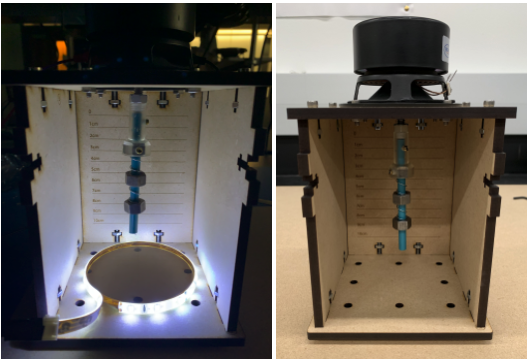
\includegraphics[width=5in]{lab4a.png}
\end{center}

\begin{enumerate}
\item First, draw a schematic illustrating how you would model the system, labelling all the masses and springs. Note that this can be modeled as a base excitation type problem.  Also clearly label the $x_1$ and $x_2$ coordinates denoting the position of the upper and lower mass, respectively.  
\begin{enumerate}
\item Write down the equations of motion for both masses, then rewrite the system in matrix form. For the purposes of the model, you should assume that the system is undamped, and that the masses and springs are identical.  The spring constant is given by the manufacturer to be around 1050 N/m, while the mass of one nut is approximately 7 g. 
\item Determine the natural frequencies and corresponding mode shapes of the 2DOF system.
\item Lastly, solve for the forced response of the two masses as a function of the driving (i.e. base excitation) frequency.  Plot the frequency response function of the upper mass (mass 1).  Correlate and label the peaks in the frequency response function to the normal modes of the system predicted in the prior part of this problem.  On the same plot, overlay the frequency response function for the 1DOF system from Lab 1 (single spring and nut case).
\item In the 2DOF system, there is also a driving frequency at which the upper mass is predicted to be completely stationary.  Calculate this special frequency.
\end{enumerate}

\item In the experiment, explore driving frequencies from 30Hz to 100Hz in order to experimentally identify the resonant frequencies (and corresponding mode shapes) as well as the special frequency at which the upper mass is nearly stationary.  Setting the strobing frequency to an offset value from the driving frequency will be very helpful for visualizing the relative amplitudes (and for the best effect, turn off the surrounding lights).  Report the experimentally determined frequencies and mode shapes and compare directly to the theoretical predictions from the previous part of this problem.  

\item Lastly, add one additional nut and spring to the end of the chain to create a 3DOF system.  Again by exploring different frequencies under strobing, identify a new qualitative response behavior.  Take a video of one these responses, and include with your assignment.  No calculations are required for this part.

\item Provide feedback or ideas (positive and/or areas for improvement) on the setup process and multi-DOF lab.

\end{enumerate}



\end{document}
